\chapter{SPIN}\label{SPIN}
\section{Spin}\label{Spin}
IN BOTH classical and quantum mechanics, the law of conservation of angular momentum is a consequence of the isotropy of space with respect to a closed system. This already demonstrates the relation between the angular momentum and the symmetry properties under rotation. In quantum mechanics, however, the relation in question is a particularly far-reaching one, and essentially constitutes the basic content of the concept of angular momentum, especially as the classical definition of the angular momentum of a particle as the product $ \bm{r}\times\bm{p} $ has no direct significance in quantum mechanics, owing to the fact that position and momentum cannot be simultaneously measured.

We have seen in \S\ref{Eigenfunctions of the angular momentum} that, if the values of $ l $ and $ m $ are specified, the angular dependence of the wave function of the particle is determined, and therefore so are all its symmetry properties under rotation. The most general formulation of these properties involves specifying the transformation of the wave functions when the coordinate system is rotated.

The wave function $\psi_{LM}$ of a system of particles (with specified values of the angular momentum $ L $ and its component $ M $) remains unchanged\footnote{Apart from an unimportant phase factor.
} only in a rotation of the coordinate system about the $ z $-axis. Any rotation that alters the direction of this axis has the result that the $ z $-component of the angular momentum does not have a definite value. This means that, in the new coordinates, the wave function in general becomes a superposition (a linear combination) of $ 2L + 1 $ functions corresponding to the different possible values of $ M $ for the given $ L $. We can say that the $ 2L + 1 $ functions $\psi_{LM}$ are transformed into linear combinations of one another when the coordinate system is rotated.\footnote{In mathematical terms, these functions are the irreducible representations of the rotation group. The number of functions which are transformed into linear combinations of one another is called the dimension of the representation; it is assumed that this number cannot be made smaller by taking any other linear combinations of these functions.
} The law governing this transformation (i.e. the coefficients in the superposition as functions of the angles of rotation of the coordinate axes) is entirely determined by specifying the value of $ L $. Thus the angular momentum acquires the significance of a quantum number which classifies the states of the system according to their transformation properties under rotation of the coordinate system. This aspect of the concept of angular momentum in quantum mechanics is particularly important because it is not directly related to the explicit angular dependence of the wave functions; the law of mutual transformation of these functions can be stated without reference to that dependence.

Let us consider a composite particle, such as an atomic nucleus, which is at rest as a whole and is in a definite internal state. In addition to an internal energy, it has also an angular momentum of definite magnitude $ L $, due to the motion of the particles within the nucleus. This angular momentum can have $ 2L + 1 $ different orientations in space. Thus, in considering the movement of a complex particle as a whole, we must assign to it, as well as its coordinates, another discrete variable: the projection of its internal angular momentum on some chosen direction in space.

However, with the preceding understanding of the concept of angular momentum, the origin of it becomes unimportant, and we naturally arrive at the concept of an “intrinsic” angular momentum which must be ascribed to the particle regardless of whether it is “composite” or “elementary”.

Thus, in quantum mechanics an elementary particle must be assigned a certain “intrinsic” angular momentum unconnected with its motion in space. This property of elementary particles is peculiar to quantum theory (it disappears in the limit $ \h\to 0 $), and therefore has in principle no classical interpretation.\footnote{In particular, it would be wholly meaningless to imagine the “intrinsic” angular momentum of an elementary particle as being the result of its rotation “about its own axis”.
}

The intrinsic angular momentum of a particle is called its \textit{spin}, as distinct from the angular momentum due to the motion of the particle in space, called the \textit{orbital angular momentum}.\footnote{The physical idea that an electron has an intrinsic angular momentum was put forward by G. Uhlenbeck and S. Goudsmit in 1925. Spin was introduced into quantum mechanics in 1927 by W. Pauli.
} The particle concerned may be either elementary, or composite but behaving in some respect as an elementary particle (e.g. an atomic nucleus). The spin of a particle (measured, like the orbital angular momentum, in units of $ \h $) will be denoted by $ s $.

For particles having spin, the description of the state by means of the wave function must determine the probability not only of its different positions in space but also of the possible orientations of the spin. Thus the wave function must depend not only on three continuous variables, the coordinates of the particle, but also on a discrete spin variable, which gives the value of the projection of the spin on a selected direction in space (the z-axis) and takes a limited number of discrete values, which we shall denote by $\sigma$.

Let $ \psi(x, y, z; \sigma) $ be such a wave function. It is essentially a set of several different functions of the coordinates, corresponding to different values of $\sigma$; these functions will be called the \textit{spin components} of the wave function. The integral
\[ \int|\psi(x,y,z;\sigma)|^2\d V \]
determines the probability that the particle has a certain value of $\sigma$. The probability that the particle is in the volume element $ \d V $ with any value of $\sigma$ is
\[ \d V\sum_{\sigma}|\psi(x,y,z;\sigma)|^2. \]



The quantum-mechanical spin operator, on being applied to the wave function, acts on the spin variable $\sigma$. In other words, it in some way linearly transforms the components of the wave function into one another. The form of this operator will be established later. However, it is easy to see from very general considerations that the operators $\hat{s}_x,\hat{s}_y,\hat{s}_z$ satisfy the same commutation conditions as the operators of the orbital angular momentum.

The angular momentum operator is essentially the same as that of an infinitely small rotation. In deriving, in \S\ref{Angular momentum}, the expression for the orbital angular momentum operator, we considered the result of applying the rotation operator to a function of the coordinates. In the case of the spin, this derivation becomes invalid, since the spin operator acts on the spin variable, and not on the coordinates. Hence, to obtain the required commutation relations, we must consider the operation of an infinitely small rotation in a general form, as a rotation of the system of coordinates. If we successively perform infinitely small rotations about the $ x $-axis and the $ y $-axis, and then about the same axes in the reverse order, it is easy to see by direct calculation that the difference between the results of these two operations is equivalent to an infinitely small rotation about the $ z $-axis (through an angle equal to the product of the angles of rotation about the $ x $ and $ y $-axes). We shall not pause here to carry out these simple calculations, as a result of which we again obtain the usual commutation relations between the operators of the components of angular momentum; these must therefore hold for the spin operators also:
\begin{equation}\label{54.1}
\{\hat{s}_y,\hat{s}_z\}=\i\hat{s}_x,\quad\{\hat{s}_z,\hat{s}_z\}=\i\hat{s}_y,\quad\{\hat{s}_x,\hat{s}_y\}=\i\hat{s}_z
\end{equation}
together with all the physical consequences resulting from them.

The commutation relations \eqref{54.1} enable us to determine the possible values of the absolute magnitude and components of the spin. All the results derived in \S\ref{Eigenvalues of the angular momentum} (formulae \eqref{27.7}–\eqref{27.9}) were based only on the commutation relations, and hence are fully applicable here also; we need only replace $ \bm{L} $ in these formulae by $ \bm{s} $. It follows from formula \eqref{27.7} that the eigenvalues of the component of the spin form a sequence of numbers differing by unity. However, we cannot now assert that these values must be integral, as we could for the component $ L_z $ of the orbital angular momentum (the derivation given at the beginning of \S\ref{Eigenvalues of the angular momentum} is invalid here, since it was based on the expression \eqref{26.14} for the operator $\hat{l}_z$, which holds only for the orbital angular momentum).

Moreover, we find that the sequence of eigenvalues $ s_z $ is limited above and below by values equal in absolute magnitude and opposite in sign, which we denote by $ \pm s $. The difference $ 2s $ between the greatest and least values of $ s_z $ must be an integer or zero. Consequently $ s $ can take the values $ 0, 1/2, 1, 3/2,\dots $

Thus the eigenvalues of the square of the spin are
\begin{equation}\label{54.2}
\bm{s}^2=s(s+1)
\end{equation}
where $ s $ can be either an integer (including zero) or half an integer. For given $ s $, the component $ s_z $ of the spin can take the values $ s, s - 1, \dots, -s $, i.e. $ 2s+1 $ values in all. Accordingly, the wave function of a particle with spin $ s $ has $ 2s + 1 $ components.\footnote{Since $ s $ is fixed for each kind of particle, the spin angular momentum $ \h s $ becomes zero in the limit of classical mechanics ($ \h\to0 $). This consideration does not apply to the orbital angular momentum, since $ l $ can take any value. The transition to classical mechanics is represented by $ \h $ tending to zero and $ l $ simultaneously tending to infinity, in such a way that the product $ \h l $ remains finite.}

Experiment shows that the majority of the elementary particles (electrons, positrons, protons, neutrons, $ \mu $-mesons and all hyperons ($ \Lambda,\Sigma,\Xi $)) have a spin of $ 1/2 $. There are also elementary particles, the $\pi$-mesons and the $ K $-mesons, whose spin is zero.

The total angular momentum of a particle is composed of its orbital angular momentum $ \bm{l} $ and its spin $ \bm{s} $. Their operators act on functions of different variables, and therefore, of course, commute. The eigenvalues of the total angular momentum
\begin{equation}\label{54.3}
\bm{j}=\bm{l}+\bm{s}
\end{equation}
are determined by the same “vector model” rule as the sum of the orbital angular momenta of two different particles (\S\ref{Addition of angular momenta}). That is, for given values of $ l $ and $ s $, the total angular momentum can take the values $ l+s, l+s- 1, \dots, |l−s| $. Thus, for an electron (spin $ 1/2 $) with non-zero orbital angular momentum $ l $, the total angular momentum can be $ j = l \pm1/2 $; for $ l = 0 $ the angular momentum $ j $ has, of course, only the one value $ j = 1/2$.

The operator of the total angular momentum $ \bm{J} $ of a system of particles is equal to the sum of the operators of the angular momentum $ \bm{j} $ of each particle, so that its values are again determined by the vector model rules. The angular momentum $ \bm{J} $ can be put in the form
\begin{equation}\label{54.4}
\bm{J}=\bm{L}+\bm{S},\quad\bm{L}=\sum_{a}\bm{l}_a,\quad\bm{S}=\sum_{a}\bm{s}_a,
\end{equation}
where $ \bm{S} $ may be called the total spin and $ \bm{L} $ the total orbital angular momentum of the system. We notice that, if the total spin of the system is half-integral (or integral), the same is true of the total angular momentum, since the orbital angular momentum is always integral. In particular, if the system consists of an even number of similar particles, its total spin is always integral, and therefore so is the total angular momentum.

The operators of the total angular momentum $ \bm{j} $ of a particle (or $ \bm{J} $, of a system of particles) satisfy the same commutation rules as the operators of the orbital angular momentum or the spin, since these rules are general commutation rules holding for any angular momentum. The formulae \eqref{27.13} for the matrix elements of angular momentum, which follow from the commutation rules, are also valid for any angular momentum, provided that the matrix elements are defined with respect to the eigenstates of this angular momentum. Formulae \eqref{29.7}—\eqref{29.10} for the matrix elements of arbitrary vector quantities also remain valid (with appropriate change of notation).





{\small
	
\textbf{PROBLEMS}


A particle with spin $ 1/2 $ is in a state with a definite value $ s_z = 1/2 $. Determine the probabilities of the possible values of the component of the spin along an axis $ z' $ at an angle $\theta$ to the $ z $-axis.





SOLUTION. The mean spin vector $ \bar{\bm{s}} $ is evidently along the $ z $-axis and has magnitude $ 1/2 $. Taking the component along the $ z' $-axis, we find that the mean value of the spin in that direction is $ \bar{s_{z'}}=(1/2)\cos\theta $. We also have $ \bar{s_{z'}}=(1/2)(w_++w_-) $ where $ w_\pm $ are the probabilities of the values $ s_{z'} = \pm1/2 $. Since $ w_++w_-= 1 $, we find 
\[ w_+ = \cos2\theta, w_- = \sin2\theta. \] }





\section{The spin operator}\label{The spin operator}
In the rest of this chapter we shall not be interested in the dependence of the wave functions on the coordinates. For example, in speaking of the behaviour of the functions $ \psi(x, y, z; \sigma) $ when the system of coordinates is rotated, we can suppose that the particle is at the origin, so that its coordinates remain unchanged by such a rotation, and the results obtained will characterize the behaviour of the function $ \psi $ with regard to the spin variable $ \sigma $.

The variable $\sigma$ differs from the ordinary variables (the coordinates) by being discrete. The most general form of a linear operator acting on functions of a discrete variable $\sigma$ is
\begin{equation}\label{55.1}
\left(\hat{f}\psi \right)(\sigma)=\sum_{\sigma'}f_{\sigma\sigma'}\psi(\sigma')
\end{equation}
where the $ f_{\sigma\sigma'} $, are constants. We put $\psi$  in parentheses in order to emphasize that the spin argument following it is not that of the original function $\psi$ but that of the function resulting from it under the action of the operator $ \hat{f} $. It is easy to see that the quantities $ f_{\sigma\sigma'} $, are the same as the matrix elements of the operator, defined by the usual rule \eqref{11.5}.\footnote{Note that the suffixes in the matrix elements on the right of \eqref{55.1} are written in an order which is, in a sense, the reverse of the usual order in \eqref{11.11}.
}

The integration over the coordinates in \eqref{11.5} is here replaced by summation over the discrete variable, so that the definition of the matrix element is
\begin{equation}\label{55.2}
f_{\sigma_2\sigma_1}=\sum_{\sigma}\psi^*_{\sigma_2}(\sigma)\left[\hat{f}\psi_{\sigma_1}(\sigma) \right]
\end{equation}
Here $ \psi_{\sigma_1}(\sigma) $ and $ \psi_{\sigma_2}(\sigma) $ are the eigenfunctions of the operator $ \hat{s}_z $ corresponding to the eigenvalues $ s_z = \sigma_1 $ and $ \sigma_2 $; each such function corresponds to a state in which the particle has a definite value of $ s_z $, i.e. in which only one component of the wave function is non-zero:\footnote{More precisely, we should write
\[ \psi_{\sigma_1}(\sigma)=\psi(x,y,z)\delta_{\sigma_1\sigma}; \]	
in \eqref{55.3} the coordinate factors are omitted, being unimportant in this connection.
	
We must once again emphasize the distinction between the specified eigenvalue $ \sigma_1 $ or $ \sigma_2 $ of $ s_z $ and the independent variable $\sigma$.
}
\begin{equation}\label{55.3}
\psi_{\sigma_1}(\sigma)=\delta_{\sigma\sigma_1},\quad\psi_{\sigma_2}(\sigma)=\delta_{\sigma\sigma_2}.
\end{equation}
According to \eqref{55.1},
\[ \left(\hat{f}\psi \right)(\sigma)=\sum_{\sigma'}f_{\sigma\sigma'}\psi_{\sigma_1}(\sigma')=\sum_{\sigma'}f_{\sigma\sigma'}\delta_{\sigma'\sigma_1}=f_{\sigma\sigma'} \]
and on substitution of this and $ \psi_{\sigma_2}(\sigma) $ the equation \eqref{55.2} is satisfied identically; this completes the proof.

Thus the operators acting on functions of $\sigma$ can be represented in the form of $ (2s + 1) $-rowed matrices. In particular, we have for the operator of the spin itself, acting on the wave function, by \eqref{55.1},
\begin{equation}\label{55.4}
\left(\hat{\bm{s}}\psi \right)(\sigma)=\sum_{\sigma'}\bm{s}_{\sigma\sigma'}\psi(\sigma')
\end{equation}
According to what has been said at the end of \S\ref{Spin}, the matrices $ \hat{s}_x, \hat{s}_y, \hat{s}_z $ are identical with the matrices $ \hat{L}_x, \hat{L}_y, \hat{L}_z $ obtained in \S\ref{Eigenvalues of the angular momentum}, where the letters $ L $ and $ M $ need only be replaced by $ s $ and $\sigma$:
\begin{equation}\label{55.5}
\begin{split}
(s_x)_{\sigma,\sigma-1}=(s_x)_{\sigma-1,\sigma}&=\frac{1}{2}\sqrt{(s+\sigma)(s-\sigma+1)},\\
(s_y)_{\sigma,\sigma-1}=-(s_y)_{\sigma-1,\sigma}&=-\frac{\i}{2}\sqrt{(s+\sigma)(s-\sigma+1)},\\
(s_z)_{\sigma\sigma}&=\sigma.
\end{split}
\end{equation}
This determines the spin operator.

In the important case of a spin of $ 1/2 $ ($ s = 1/2, σ = \pm1/2 $), these matrices have two rows, and are of the form
\begin{equation}\label{55.6}
\hat{\bm{s}}=\frac{1}{2}\hat{\bm{\sigma}}
\end{equation}
where\footnote{In the tabular matrices \eqref{55.7} the rows and columns are numbered by the values of σ, the row number corresponding to the first and the column number to the second suffix of the matrix element. In the present case, these numbers are $ +1/2 $ and $ -1/2 $. The action of the. operator shown by \eqref{55.4} multiplies row $\sigma$ of the matrix by a column matrix containing the components of the wave function:
	\[ \psi=\left(\begin{array}{c}
	\psi(1/2)\\
	\psi(-1/2)
	\end{array}\right) \]
}
\begin{equation}\label{55.7}
\hat{\bm{\sigma}}_x=\left(\begin{array}{cc}
0&1\\
1&0
\end{array} \right),\quad\hat{\bm{\sigma}}_y=\left( \begin{array}{cc}
0&-\i\\\i&0
\end{array}\right),\quad
\hat{\bm{\sigma}}_z=\left(\begin{array}{cc}
1&0\\
0&-1
\end{array} \right).
\end{equation}


These are called \textit{Pauli matrices}. The matrix $ \hat{\bm{s}}_z=\frac{\hat{\bm{\sigma}}_z}{2} $ is diagonal, as it should be, since it is defined in terms of the eigenfunctions of the quantity $ \bm{s}_z $ itself.\footnote{There should be no misunderstanding because of the use of the same letter to denote the spin component and the Pauli matrices, since the latter always have the circumflex.
}

The following are some specific properties of the Pauli matrices. Direct multiplication of the matrices \eqref{55.7} gives the equations
\begin{equation}\label{55.8}
\begin{split}
\hat{\bm{\sigma}}_x^2=\hat{\bm{\sigma}}_y^2&=\hat{\bm{\sigma}}_z^2=1\\
\hat{\bm{\sigma}}_y\hat{\bm{\sigma}}_z=\i\hat{\bm{\sigma}}_x,\quad\hat{\bm{\sigma}}_z\hat{\bm{\sigma}}_x&=\i\hat{\bm{\sigma}}_y,\quad\hat{\bm{\sigma}}_x\hat{\bm{\sigma}}_y=\i\hat{\bm{\sigma}}_z
\end{split}
\end{equation}
Combining these with the general commutation rules \eqref{54.1}, we find that
\begin{equation}\label{55.9}
\hat{\bm{\sigma}}_\i\hat{\bm{\sigma}}_k+\hat{\bm{\sigma}}_k\hat{\bm{\sigma}}_\i=2\delta_{\i k}
\end{equation}
i.e. the Pauli matrices anticommute with one another. By means of these equations, we can easily verify the following useful formulae:
\begin{equation}\label{55.10}
\hat{\bm{\sigma}}^2=3,\quad (\hat{\bm{\sigma}}\cdot\bm{a})(\hat{\bm{\sigma}}\cdot\bm{b})=\bm{a}\cdot\bm{b}+\i\hat{\bm{\sigma}}\cdot\bm{a}\times\bm{b}.
\end{equation}
where $ \bm{a} $ and $ \bm{b} $ are any vectors.\footnote{The terms on the right of \eqref{55.8}–\eqref{55.10} which are independent of $\hat{\bm{\sigma}}$ must, of course, be understood as constants multiplying the unit two-by-two matrix.
} According to these relations, any scalar polynomial formed from the matrices $ \hat{\bm{\sigma}}_i $ can be reduced to terms independent of $ \hat{\bm{\sigma}} $ and terms linear in $ \hat{\bm{\sigma}} $; hence it follows that any scalar function of the operator ∂ reduces to a linear function (see Problem 1). Lastly, the values of the traces (sums of diagonal elements) of the Pauli matrices and their products are
\begin{equation}\label{55.11}
\mathrm{tr}\hat{\sigma}_i=0,\quad\mathrm{tr}\hat{\sigma}_i\hat{\sigma}_k=2\delta_{ik}.
\end{equation}


Subsequent sections of this chapter give a more detailed account of the spin properties of wave functions, including their behaviour under any rotation of the coordinate system, but we may note immediately an important property of these functions, namely their behaviour in respect of rotations about the $ z $-axis.

Let there be an infinitesimal rotation through an angle $ \delta\phi $ about the $ z $-axis. The operator of such a rotation is expressed in terms of the angular momentum operator (in this case, the spin operator) as $ 1 + \i \delta\phi\cdot\hat{s}_z $. As a result of the rotation, the functions $ \psi(\sigma) $ therefore become $ \psi(\sigma) + \delta\psi(\sigma) $, where
\[ \delta\psi(\sigma)=\i\delta\phi\cdot\hat{s}_z\psi(\sigma)=\i\sigma\psi(\sigma)\delta\phi \]



Writing this relation in the form $ \d\psi/\d\phi = \i\sigma\psi(\sigma) $ and integrating, we find that a rotation through a finite angle $\phi$ changes the functions $\psi(\sigma)$ into
\begin{equation}\label{55.12}
\psi(\sigma)'=\psi(\sigma)\e^{\i\sigma\phi}
\end{equation}
In particular, a rotation through $ 2\pi $ multiplies them by a factor $ \e^{2\pi\i\sigma} $, which is the same for all $\sigma$ and is equal to $ (-1)^{2s} $ (since $ 2\sigma $ always has the same parity as $ 2s $). Thus, in a complete rotation of the coordinate system about the $ z $-axis, the wave functions of particles with integral spin return to their original values, and those of particles with half-integral spin change sign.





{\small
\textbf{PROBLEMS}


\textbf{1.} Reduce an arbitrary function of the scalar $ a + \bm{b}\cdot\hat{\bm{\sigma}} $ linear in the Pauli matrices to another linear function.





SOLUTION. TO determine the coefficients in the required formula
\[  f (a + \bm{b}\cdot\hat{\bm{\sigma}}) = \bm{A}+\bm{B}\hat{\bm{\sigma}},  \]
we note that, when the $ z $-axis is taken in the direction of $ \bm{b} $, the eigenvalues of the operator $ a + \bm{b}\cdot\hat{\bm{\sigma}} $ are $ a \pm b $, and the corresponding eigenvalues of the operator $ f (a + \bm{b}\cdot\hat{\bm{\sigma}})  $ are $ f (a \pm b) $. Hence we find 
\[ A = \frac{1}{2}[f (a + b) + f (a − b)], \bm{B} = \frac{\bm{b}}{2b} [f (a + b)-f (a−b)]. \]





\textbf{2.} Determine the values of the scalar product $ \bm{S}_1\cdot\bm{S}_2 $ of spins ($ 1/2 $) of two particles in states in which the total spin of the system, $ \bm{S} = \bm{s}_1 + \bm{s}_2 $, has definite values ($ 0 $ or $ 1 $).





SOLUTION. From the general formula \eqref{31.3}, which is valid for the addition of any two angular momenta, we find 
\[ \bm{s}_1\cdot \bm{s}_2 = 1/4\text{ for }S = 1,\quad \bm{s}_1\cdot \bm{s}_2 = -3/4\text{ for }S = 0. \]





\textbf{3.} Which powers of the operator ŝ of an arbitrary spin $\hat{\bm{s}}$ are independent?





SOLUTION. The operator
\[ (\hat{s}_z-s)(\hat{s}_z-s+1)\dots(\hat{s}_z+s), \]
formed from the differences between $\hat{s}_z$ and all possible eigenvalues $ s_z $, gives zero when it is applied to any wave function, and is therefore itself zero. Hence it follows that $ (\hat{s}_z)^{2s+1} $ is expressed in terms of lower powers of the operator $\hat{s}_z$, so that only its powers from $ 1 $ to $ 2s $ are independent.}
\section{Spinors}\label{Spinors}
When the spin is zero, the wave function has only one component, $ \psi(0) $. The effect of the spin operator is to reduce it to zero: $ \hat{\bm{s}}\psi= 0 $. The relation between $ \hat{\bm{s}} $ and the operator of an infinitesimal rotation implies that the wave function of a particle with zero spin is invariant under rotation of the coordinate system, i.e. it is a scalar.

The wave function of a particle with spin $ 1/2 $ has two components, $ \psi(1/2) $ and $ \psi(-1/2) $. For convenience in later generalizations, we shall distinguish these components by the superscripts $ 1 $ and $ 2 $ respectively. The two-component quantity
\begin{equation}\label{56.1}
\psi=\left(\begin{array}{c}
\psi^1\\\psi^2
\end{array} \right)\equiv\left(\begin{array}{c}
\psi\left(1/2\right)\\\psi\left(-1/2\right)
\end{array} \right)
\end{equation}
is called a \textit{spinor}.

In any rotation of the coordinate system, the components of the spinor undergo a linear transformation:
\begin{equation}\label{56.2}
\psi^{1'}=a\psi^1+b\psi^2,\quad\psi^{2'}=c\psi^1+d\psi^2.
\end{equation}
This may be written
\begin{equation}\label{56.3}
\psi^{\lambda'}=(\hat{U}\psi)^\lambda,\quad\hat{U}=\left(\begin{array}{cc}
a&b\\
c&d
\end{array}\right),
\end{equation}
where $\hat{U}$ is the transformation matrix.\footnote{The notation $ \hat{U}\psi $ implies that the rows of the matrix $\hat{U}$ are multiplied by the column $\psi$.} Its elements are in general complex functions of the angles of rotation of the coordinate axes. They are connected by relations which follow directly from the physical conditions imposed on the spinor as the wave function of a particle.

Let us consider the bilinear form
\begin{equation}\label{56.4}
\psi^1\phi^2-\psi^2\phi^1,
\end{equation}
where $\psi$ and $\phi$ are two spinors. A simple calculation gives
\[ \psi^{1'}\phi^{2'}-\psi^{2'}\phi^{1'}=(ad-bc)(\psi^1\phi^2-\psi^2\phi^1), \]
i.e. \eqref{56.4} is transformed into itself when the coordinate system is rotated. If, however, there is only one function which is transformed into itself, it can be regarded as corresponding to zero spin, and therefore must be a scalar, i.e. must remain unchanged when the coordinate system is rotated in any manner. Hence we have
\begin{equation}\label{56.5}
ad-bc=1;
\end{equation}
the determinant of the transformation matrix is unity.\footnote{Such a transformation of two quantities is called a \textit{binary transformation}.}

Further relations follow from the requirement that the expression
\begin{equation}\label{56.6}
\psi^1\psi^{1*}+\psi^2\psi^{2*},
\end{equation}
which determines the probability of finding the particle at a given point in space, should be a scalar. A transformation which leaves unchanged the sum of the squared moduli of the quantities is a unitary transformation, i.e. we must have $ \hat{U}^\dagger=\hat{U}^{-1} $ (see \S\ref{Transformation of matrices}). With the condition \eqref{56.5} the inverse matrix is
\[ \hat{U}^{-1}=\left(\begin{array}{cc}
d&-b\\
-c&a
\end{array}\right). \]
Equating this to the Hermitian conjugate matrix
\[ \hat{U}^\dagger=\left(\begin{array}{cc}
a^*&c^*\\
b^*&d^*
\end{array}\right), \]
we find
\begin{equation}\label{56.7}
a=d^*,\quad b=-c^*
\end{equation}


By virtue of the relations \eqref{56.5} and \eqref{56.7}, the four complex quantities $ a, b, c, d $ actually contain only three independent real parameters, corresponding to the three angles which define a rotation of a three-dimensional system of coordinates.

Comparison of the expressions for the scalars \eqref{56.4} and \eqref{56.6} shows that $\psi^{1*}$ and $\psi^{2*}$ must be transformed as $\psi^2$ and $ -\psi^1 $ respectively. It is easy to verify that this is in fact so, using \eqref{56.5} and \eqref{56.7}.\footnote{This property is closely associated with symmetry under time reversal. The latter (see \S\ref{The fundamental properties of Schr\"odinger's equation}) involves the replacement of the wave function by its complex conjugate. Under time reversal, the angular momentum components also change sign. Hence the functions that are the complex conjugates of the components $ \psi^1 \equiv \psi(1/2) $ and $ \psi^2 \equiv \psi(-1/2) $ must have properties equivalent to those of the components corresponding to spin projections $ -1/2 $ and $ 1/2 $ respectively.
}

It is possible to put the algebra of spinors in a form analogous to that of tensor algebra. This is done by introducing, in addition to \textit{contravariant} spinor components $ \psi^1, \psi^2 $ (with superscripts), the \textit{covariant} components (with subscripts), defined by
\begin{equation}\label{56.8}
\psi_1=\psi^2,\quad\psi_2=-\psi^1
\end{equation}
The invariant combination \eqref{56.4} of the two spinors may also be written as a scalar product
\begin{equation}\label{56.9}
\psi^\lambda\phi_\lambda=\psi^1\phi_1+\psi^1\phi_2-\psi^2\phi_1;
\end{equation}
here and below, summation over repeated (\textit{dummy}) indices is implied, as in tensor algebra. We may note the following rule which has to be borne in mind in spinor algebra. We have
\[ \psi^\lambda\phi_\lambda=\psi^1\phi_1+\psi^2\phi_2=-\psi_2\phi^2-\psi_1\phi^1. \]
Thus
\begin{equation}\label{56.10}
\psi^\lambda\phi_\lambda=-\psi_\lambda\phi^\lambda
\end{equation}
Hence it is evident that the scalar product of any spinor with itself is zero:
\begin{equation}\label{56.11}
\psi^\lambda\psi_\lambda=0.
\end{equation}


According to the foregoing discussion, the quantities $\psi_1$ and $\psi_2$ are transformed as $ \psi^{1*} $ and $ \psi^{2*} $, i.e.
\begin{equation}\label{56.12}
\psi_\lambda'=\left(\hat{U}^*\psi \right)_\lambda
\end{equation}


The product $ \hat{U}^*\psi $ may also be written as $ \psi\tilde{\hat{U}^*} $, with the transposed matrix $\tilde{\hat{U}^*}$. Since $\hat{U}$ is unitary, we have $ \tilde{\hat{U}^*}=\hat{U}^{-1} $, so that $ \psi_\lambda'=\left(\psi\hat{U}^{-1}\right)_\lambda $ or\footnote{The notation $\psi\hat{U}$ (with $\psi$ to the left of $\hat{U}$) denotes that the components ($ \psi_1\psi_2 $) as a row are multiplied by the columns of the matrix $\hat{U}$.
}
\begin{equation}\label{56.13}
\psi_\lambda=\left(\psi'\hat{U} \right)_\lambda
\end{equation}


Analogously to the transition from vectors to tensors in ordinary tensor algebra, we can introduce the idea of spinors of higher rank. Thus, a quantity $\psi^{\lambda\mu}$, having four components which are transformed as the products $ \psi^\lambda\phi^\mu $ of the components of two spinors of rank one, is called a spinor of rank two. Besides the contra variant components $\psi^{\lambda\mu}$ we can consider the covariant components $\psi^{\lambda\mu}$ and the mixed components $ \psi^{\mu}_\lambda $ which are transformed as the products $ \psi_\lambda\phi_mu $ and $ \psi_\lambda\phi^\mu $ respectively. Spinors of any rank are similarly defined.

The transition from contravariant to covariant spinor components and \textit{vice versa} may be written
\begin{equation}\label{56.14}
\psi_\lambda=g_{\\lambd
\mu}\psi^\mu,\quad\psi^\lambda=g^{\mu\lambda}\psi_mu,
\end{equation}
where
\begin{equation}\label{56.15}
\left(g_{\lambda\mu}\right)=\left(g^{\lambda\mu}\right)=\left(\begin{array}{cc}
0&1\\-1&0
\end{array}\right)
\end{equation}
is the \textit{metric spinor} in a vector space of two dimensions. Thus we have, for example,
\[ \psi_\lambda^\mu=g_{\lambda\nu}\psi^{\nu\mu},\quad\psi_{\lambda\mu}=g_{\lambda\nu}g_{\mu\rho}\psi^{\nu\rho} \]
so that $ \psi_{12} = -\psi_1^{\text{ }1} = -\psi^{21}, \psi_{11} = \psi_1^{\text{ }2} = \psi^{22} $, and so on.

The quantities $ g_{\lambda\mu} $ themselves form an antisymmetric unit spinor of rank two. It is easy to see that the values of its components remain unchanged under transformations of the coordinates, and that
\begin{equation}\label{56.16}
g_{\lambda\nu}g^{\mu\nu}=\delta_\lambda^\mu
\end{equation}
where $ \delta_1^1 = \delta_2^2 = 1, \delta_2^1 = \delta_1^2 = 0 $.

As in ordinary tensor algebra, there are two fundamental operations in spinor algebra: multiplication, and contraction with respect to a pair of indices. The \textit{multiplication} of two spinors gives a spinor of higher rank; thus, from two spinors of ranks two and three, $\psi_{\lambda\mu}$ and $ \psi^{\nu\rho\sigma} $, we can form a spinor of rank five, $\psi_{\lambda\mu}\psi^{\nu\rho\sigma}  $. \textit{Contraction} with respect to a pair of indices (i.e. summation of the components over corresponding values of one covariant and one contravariant index) decreases the rank of a spinor by two. Thus, a contraction of the spinor $ \psi_{\lambda\mu}{}^{\nu\rho\sigma} $ with respect to the indices $\mu$ and $\nu$ gives the spinor  $\psi_{\lambda\mu}{}^{\mu\rho\sigma} $ of rank three; the contraction of the spinor $ \psi_\lambda{}^{\mu} $ gives the scalar $ \psi_\lambda{}^{\lambda} $. Here there is a rule similar to that expressed by formula \eqref{56.10}: if we interchange the upper and lower indices with respect to which the contraction is effected, the sign is changed (i.e. $ \psi_\lambda{}^{\lambda}=-\psi^\lambda{}_{\lambda} $). Hence, in particular, it follows that, if a spinor is symmetrical with respect to any two of its indices, the result of a contraction with respect to these indices is zero. Thus, for a symmetrical spinor $ \psi_{\lambda\mu} $ of rank two, we have $ \psi_\lambda{}^\lambda = 0 $.

A spinor of rank $ n $ symmetrical with respect to all its indices is called a \textit{symmetrical spinor} of rank $ n $. From an asymmetrical spinor we can construct a symmetrical one by the process of \textit{symmetrization}, i.e. summation of the components obtained by all possible interchanges of the indices. From what has been said above, it is impossible to construct (by contraction) a spinor of lower rank from the components of a symmetrical spinor.

Only a spinor of rank two can be antisymmetrical with respect to all its indices. For, since each index can take only two values, at least two out of three or more indices must have the same value, and therefore the components of the spinor are zero identically. Any antisymmetrical spinor of rank two is a scalar multiple of the unit spinor $ g_{\lambda\mu} $. We may notice here the following relation:
\begin{equation}\label{56.17}
g_{\lambda\mu}\psi_\nu+g_{\mu\nu}\psi_\lambda+g_{\nu\lambda}\psi_\mu=0
\end{equation}
(where $\psi_\lambda$ is any spinor), which follows from the above; this rule is simply a consequence of the fact that the expression on the left is (as we may easily verify) an antisymmetrical spinor of rank three.

The spinor which is the product of a spinor $\psi_{\lambda\mu}$ with itself, on contraction with respect to one pair of indices, becomes antisymmetrical with respect to the other pair:
\[ \psi_{\lambda\nu}\psi_\mu{}^\nu=-\psi_\lambda{}^\nu\psi_{\mu\nu}. \]
Hence, from what was said above, this spinor must be a scalar multiple of the spinor $ g_{\lambda\mu} $. Defining the scalar factor so that contraction with respect to the second pair of indices gives the correct result, we find
\begin{equation}\label{56.18}
\psi_{\lambda\nu}\psi_nu{}^\nu=-(1/2)\psi_{\rho\sigma}\psi^{\rho\sigma}g_{\lambda\mu}
\end{equation}


The components of the spinor $\psi_{\lambda\mu\dots}{}^*$ which is the complex conjugate of $ \psi_{\lambda\mu\dots} $ are transformed as the components of a contravariant spinor $ \phi^{\lambda\mu\dots} $, and conversely. The sum of the squared moduli of the components of any spinor is consequently invariant.

\section{The wave functions of particles with arbitrary spin}\label{The wave functions of particles with arbitrary spin}
Having developed a formal algebra for spinors of any rank, we can now turn to our immediate problem, to study the properties of wave functions of particles with arbitrary spin.

This subject is conveniently approached by considering an assembly of $ n $ particles with spin $ 1/2 $. The greatest possible value of the $ z $-component of the total spin is $ n/2 $, which is obtained when $ s_z = 1/2 $ for every particle (i.e. all the spins are directed the same way, along the $ z $-axis). In this case we can evidently say that the total spin $ S $ of the system is also $ n/2 $.

All the components of the wave function $ \psi(\sigma_1, \sigma_2, \dots, \sigma_n) $ of the system of particles are then zero, except for $ \psi(1/2, 1/2, \dots,1/2) $. If we write the wave function as a product of $ n $ spinors $ \psi^\lambda\psi^\mu\dots $, each of which refers to one of the particles, only the component with $ \lambda, \mu,\dots = 1 $ in each spinor is not zero. Thus only the product $ \psi^1\phi^1 $ is not zero. The set of all these products, however, is a spinor of rank $ n $ which is symmetrical with respect to all its indices. If we transform the coordinate system (so that the spins are not directed along the $ z $-axis), we obtain a spinor of rank $ n $, general in form except that it is symmetrical as before.

The spin properties of wave functions, being essentially their properties with respect to rotations of the coordinate system, are identical for a particle with spin $ s $ and for a system of $ n = 2s $ particles each with spin $ 1/2 $ directed so that the total spin of the system is $ s $. Hence we conclude that the wave function of a particle with spin $ s $ is a symmetrical spinor of rank $ n = 2s $.

It is easy to see that the number of independent components of a symmetrical spinor of rank $ 2s $ is equal to $ 2s + 1 $, as it should be. For all those components are the same whose indices include $ 2s $ ones and $ 0 $ twos; so are all those with $ 2s−1 $ ones and $ 1 $ two, and so on up to $ 0 $ ones and $ 2s $ twos.

Mathematically, the symmetrical spinors provide a classification of the possible types of transformation of quantities when the coordinate system is rotated. If there are $ 2s + 1 $ different quantities which are transformed linearly into one another (and which cannot be reduced in number by any choice of linear combinations of them), then we can assert that their law of transformation is equivalent to that of the components of a symmetrical spinor of rank $ 2s $. Any set of any number of functions which are transformed linearly into one another when the coordinate system is rotated can be reduced (by an appropriate linear transformation) to one or more symmetrical spinors.\footnote{In other words, the symmetrical spinors form what are called irreducible representations of the rotation group (see \S98).
}

Thus an arbitrary spinor $ \psi_{\lambda\mu\nu} $ of rank $ n $ can be reduced to symmetrical spinors of ranks $ n, n-2, n-4, \dots $. In practice, such a reduction can be made as follows. By symmetrizing the spinor $ \psi_{\lambda\mu\nu} $ with respect to all its indices, we form a symmetrical spinor of the same rank $ n $. Next, by contracting the original spinor $ \psi_{\lambda\mu\nu} $ with respect to various pairs of indices, we obtain spinors of rank $ n - 2 $, of the form $ \psi^\lambda{}_{\lambda\nu\dots} $, which, in turn, we symmetrize, so that symmetrical spinors of rank $ n-2 $ are obtained. By symmetrizing the spinors obtained by contracting $ \psi_{\lambda\mu\dots} $ with respect to two pairs of indices, we obtain symmetrical spinors of rank $ n-4 $, and so on.

We have still to establish the relation between the components of a symmetrical spinor of rank $ 2s $ and the $ 2s + 1 $ functions $ \psi(\sigma) $, where $ \sigma= s, s - 1, \dots, -s $. The component
\[ \psi^{\underbrace{11\dots1}_{s+\sigma}\overbrace{22\dots2}^{s+\sigma}}, \]
in whose indices $ 1 $ occurs $ s + \sigma $ times and $ 2 $ $ s - \sigma $ times, corresponds to a value $\sigma$ of the projection of the spin on the $ z $-axis. For, if we again consider a system of $ n = 2s $ particles with spin $ 1/2 $, instead of one particle with spin $ s $, the product corresponds to the above component
\[ \overbrace{\psi^1\phi^1\dots}^{s+\sigma}\overbrace{\chi^2\rho^2}^{s-\sigma} \]
this product belongs to a state in which $ s + \sigma $ particles have a projection of the spin equal to $ +1/2 $, and $ s -σ $ a projection of $ -1/2 $, so that the total projection is $ 1/2(s + \sigma) - 1/2(s -\sigma) = \sigma $. Finally, the proportionality coefficient between the above component of the spinor and $ \psi(\sigma) $ is chosen so that the equation
\begin{equation}\label{57.1}
\sum_{\sigma=-s}^{+s}|\psi(\sigma)|^2=\sum_{\lambda,\mu,\dots=1}^{2}|\psi^{\lambda\mu\dots}|^2
\end{equation}
holds; this sum is a scalar, as it should be, since it determines the probability of finding the particle at a given point in space. In the sum on the right-hand side, the components with $ (s + \sigma) $ indices $ 1 $ occur
\[ \frac{(2s)!}{(s+\sigma)!(s-\sigma)!} \]
times. Hence it is clear that the relation between the functions $ \psi(\sigma) $ and the components of the spinor is given by the formula
\begin{equation}\label{57.2}
\psi(\sigma)=\sqrt{\frac{(2s)!}{(s+\sigma)!(s-\sigma)!}}\psi^{\underbrace{11\dots1}_{s+\sigma}\overbrace{22\dots2}^{s-\sigma}}
\end{equation}


The relation \eqref{57.2} ensures the fulfilment not only of the condition \eqref{57.1}, but also, as we easily see, of the more general condition
\begin{equation}\label{57.3}
\psi^{\lambda\mu\dots}\phi_{\lambda\mu\dots}=\sum_{\sigma}(-1)^{s-\sigma}\psi(\sigma)\phi(-\sigma),
\end{equation}
where $ \psi^{\lambda\mu\dots} $ and $\phi_{\lambda\mu\dots}$ are two different spinors of the same rank, while $ \psi(\sigma) $, $ \phi(\sigma) $ are functions derived from these spinors by formula \eqref{57.2}; the factor $ (-1)^{s-\sigma} $ is due to the fact that, when all the indices of the spinor components are raised, the sign changes as many times as there are twos among the indices.

Formulae \eqref{55.5} determine the result of the action of the spin operator on the wave functions $\psi(\sigma)$. It is not difficult to find how these operators act on a wave function written in the form of a spinor of rank $ 2s $. For a spin $ 1/2 $, the functions $ \psi(+1/2) $, $ \psi(-1/2) $ are the same as the components $\psi^1$, $ \psi^2 $ of the spinor. According to \eqref{55.6} and \eqref{55.7}, the result of the spin operators’ acting on them will be
\begin{equation}\label{57.4}
\begin{split}
(\hat{s}_x\psi)^1&=(1/2)\psi^2,\quad(\hat{s}_y\psi)^1=-(\i/2)\psi^2,\quad(\hat{s}_z\psi)^1=(1/2)\psi^1,\\
(\hat{s}_x\psi)^2&=(1/2)\psi^1,\quad(\hat{s}_y\psi)^2=(\i/2)\psi^1,\quad(\hat{s}_x\psi)^2=-(1/2)\psi^2.
\end{split}
\end{equation}


To pass to the general case of arbitrary spin, we again consider a system of $ 2s $ particles with spin $ 1/2 $, and write its wave function as a product of $ 2s $ spinors. The spin operator of the system is the sum of the spin operators of each particle, acting only on the corresponding spinor, the result of this action being given by formulae \eqref{57.4}. Next, returning to arbitrary symmetrical spinors, i.e. to the wave functions of a particle with spin $ s $, we obtain
\begin{equation}\label{57.5}
\begin{split}
(\hat{s}_x\psi)^{\overbrace{11\dots}^{s+\sigma}\overbrace{22\dots}^{s-\sigma}}&=\frac{s+\sigma}{2}\psi^{\overbrace{11\dots}^{s+\sigma-1}\overbrace{22\dots}^{s-\sigma+1}}+\frac{s-\sigma}{2}\psi^{\overbrace{11\dots}^{s+\sigma+1}\overbrace{22\dots}^{s-\sigma-1}},\\
(\hat{s}_y\psi)^{\overbrace{11\dots}^{s+\sigma}\overbrace{22\dots}^{s-\sigma}}&=-\i\frac{s+\sigma}{2}\psi^{\overbrace{11\dots}^{s+\sigma-1}\overbrace{22\dots}^{s-\sigma+1}}+\i\frac{s-\sigma}{2}\psi^{\overbrace{11\dots}^{s+\sigma+1}\overbrace{22\dots}^{s-\sigma-1}},\\
(\hat{s}_z\psi)^{\overbrace{11\dots}^{s+\sigma}\overbrace{22\dots}^{s-\sigma}}&=\sigma\psi^{\overbrace{11\dots}^{s+\sigma}\overbrace{22\dots}^{s-\sigma}}.
\end{split}
\end{equation}
Hitherto we have spoken of spinors as wave functions of the intrinsic angular momentum of elementary particles. Formally, however, there is no difference between the spin of a single particle and the total angular momentum of any system regarded as a whole, neglecting its internal structure. It is therefore evident that the transformation properties of spinors apply equally to the behaviour, with respect to rotations in space, of the wave functions $\psi_{jm}$ of any particle or system of particles with total angular momentum $ j $, independent of whether orbital or spin angular momentum is concerned. There must therefore be some definite relation between the laws of transformation for the eigenfunctions $\psi_{jm}$ under rotations of the coordinate system and those for the components of a symmetrical spinor of rank $ 2j $.

In establishing this relation we must, however, make a clear distinction between two aspects of the dependence of the wave functions on the component $ m $ (for a given value of $ j $). The wave function may be regarded as the probability amplitude for various values of $ m $, or may be considered for a given value of $ m $.

These two aspects have already been discussed at the beginning of \S\ref{The spin operator}, where we dealt with the eigenfunction $ \delta_{\sigma\sigma_0} $ of the operator $ \hat{s}_z $ which corresponds to $ s_z = \sigma_0 $. The mathematical difference between them is especially clear for a particle of spin $ s = 1/2 $. In this case the spin function is, with respect to the variable $\sigma$, a contravariant spinor of rank $ 1 $, i.e. must be written in spinor notation as $\delta^\sigma_{\sigma_0}$. With respect to $\sigma_0$ it is therefore a covariant spinor.

This is evidently a general result: the eigenfunctions $\psi_{jm}$ can be put in correspondence with the components of a covariant symmetrical spinor of rank $ 2j $ by means of formulae analogous to \eqref{57.2}:\footnote{This result can also be regarded somewhat differently. If the wave function $\psi$ of a particle in a state with angular momentum $ j $ is expanded in terms of the eignfunctions $\psi_{jm}$:
\[ \psi=\sum_{m}a_m\psi_{jm}, \]
then the coefficients $ a_m $ are the probability amplitudes for various values of $ m $. In this sense they correspond to the “components” $ \psi(m) $ of a spin wave function, and this gives their law of transformation. On the other hand, the value of $\psi$ at a given point in space cannot depend on the choice of the coordinate system, i.e. the sum $ \sum a_m\psi_{jm} $ must be a scalar. Comparing with the scalar \eqref{57.3}, we see that $ a_m $ must transform as $ (-1)^{j-m}\psi_{j,-m} $.}
\begin{equation}\label{57.6}
\psi_{jm}=\sqrt{\frac{(2j)!}{(j+m)!(j-m)!}}\psi_{\underbrace{11\dots}_{j+m}\underbrace{22\dots}_{j-m}}.
\end{equation}


The eigenfunctions of integral angular momentum $ j $ are spherical harmonics $ Y_{jm} $. The case $ j = 1 $ is of particular importance. The three spherical harmonics $ Y_{1m} $ are
\[ Y_{10}=\i\sqrt{\frac{3}{4\pi}}\cos\theta=\i\sqrt{\frac{3}{4\pi}}n_z, \]
\[ Y_{1,\pm1}=\mp\i\sqrt{\frac{3}{8\pi}}\sin\theta\cdot\e^{\pm\i\phi}=\mp\i\sqrt{\frac{3}{8\pi}}(n_x\pm\i n_y) \]
where $ \bm{n} $ is a unit vector along the radius vector. It is seen that these three functions are equivalent, as regards their transformation properties, to the components of a vector $ \bm{a} $, with the relations
\begin{equation}\label{57.7}
\psi_{10}=\i a_z,\quad\psi_{11}=-\frac{\i}{\sqrt{2}}(a_x+\i a_y),\quad\psi_{1,-1}=\frac{\i}{\sqrt{2}}(a_x-\i a_y).
\end{equation}
Comparing with \eqref{57.6}, we see that the components of a symmetrical spinor of rank two can be brought into correspondence with the components of thevector by the formulae
\begin{equation}\label{57.8}
\psi_{12}=\frac{\i}{\sqrt{2}}a_z,\quad\psi_{11}=-\frac{\i}{\sqrt{2}}(a_x+\i a_y),\quad\psi_{22}=\frac{\i}{\sqrt{2}}(a_x-\i a_y),\end{equation}
\begin{equation}\label{57.9}
\psi^{12}=-\frac{\i}{\sqrt{2}}a_z,\quad\psi^{11}=\frac{\i}{\sqrt{2}}(a_x-\i a_y),\quad\psi^{22}=-\frac{\i}{\sqrt{2}}(a_x+\i a_y).
\end{equation}
Conversely
\begin{equation}\label{57.10}
a_z=\i\sqrt{2}\psi^{12},\quad a_x=\frac{\i}{\sqrt{2}}(\psi^{22}-\psi^{11}),\quad a_y=\frac{1}{\sqrt{2}}(\psi^{11}+\psi^{22}).
\end{equation}


It is easily verified that with these definitions we have
\begin{equation}\label{57.11}
\psi_{\lambda\mu}\phi^{\lambda\mu}=\bm{a}\bm{b}
\end{equation}
where $ \bm{a} $ and $ \bm{b} $ are vectors corresponding to the symmetrical spinors $\psi^{\lambda\mu}$ and $ \phi^{\lambda\mu} $. It is also not difficult to see that there is a correspondence between the spinor and the vector\footnote{The mixed components of a symmetrical spinor may be written in the form $ \psi^\lambda_{\mu} $, without distinction between $\psi^\lambda{}_{\mu}$ and $\psi_\mu{}^\lambda$.
}
\begin{equation}\label{57.12}
\psi^\lambda_\nu\phi^{\mu\nu}+\psi^\mu_\nu\phi^{\lambda\nu}\text{ and }\sqrt{2}\bm{a}\times\bm{b}.
\end{equation}
Formulae \eqref{57.10} may be compactly written by means of the Pauli matrices:
\begin{equation}\label{57.13}
\bm{a}=\frac{\i}{\sqrt{2}}\bm{\sigma}^\lambda{}_\mu\phi^\mu_\lambda\quad\phi^\mu_\lambda=-\frac{\i}{\sqrt{2}}\bm{a}\cdot\bm{\sigma}^\mu_\lambda
\end{equation}
the matrix indices of $ \hat{\bm{\sigma}} $ are written as superscript and subscript in correspondence with the position of the spinor indices in $\psi^\mu_\lambda$. The origin of this formula is easily understood by considering the particular case where the spinor of rank two $\psi^\mu_\lambda$ reduces to a product of a spinor of rank one $\psi^\mu$ and its complex conjugate $ \psi^{\lambda*} $. Then the quantity
\[ \frac{1}{2}\psi^{\lambda*}\bm{\sigma}^\mu{}_\lambda\psi^\nu \] 
is the mean value of the spin (for a particle with wave function $\psi^mu$) and it is therefore evidently a vector.

The relations \eqref{57.8} or \eqref{57.9} are a particular case of a general rule: any symmetrical spinor of even rank $ 2j $, where $ j $ is integral, can be correlated with a symmetrical tensor of half the rank ($ j $) which gives zero on contraction with respect to any pair of indices; we call this an \textit{irreducible tensor}.

This follows from the fact that the numbers of independent components of the spinor and of the tensor are the same ($ 2j + 1 $), as may easily be seen.\footnote{We can say that the $ 2j + 1 $ components of an irreducible tensor of rank $ j $ (an integer), the $ 2j + 1 $ spherical harmonics Yjm, and the $ 2j + 1 $ components of a symmetrical spinor of rank $ 2j $ give the same irreducible representation of the rotation group.} The relation between the components of the spinor and of the tensor can be found by means of formulae \eqref{57.8}–\eqref{57.10}, if we consider a spinor of the rank concerned as the product of several spinors of rank two, and the tensor as a product of vectors.





{\small
	
\textbf{PROBLEMS}


\textbf{1.} Rewrite the definition \eqref{57.4} of the operator of spin $ 1/2 $ in terms of the spinor components of the vector $\hat{s}$.





SOLUTION. By means of formulae \eqref{57.9}, which give the relation between the vector $\hat{s}^{\lambda\mu}$ and the spinor $\hat{s}^{\lambda\mu}$, the definition \eqref{57.4} can be written as
\[ \hat{s}^{\lambda\mu}\psi^\nu=\frac{\i}{2\sqrt{2}}(\psi^\lambda g^{\mu\nu}+\psi^\mu g^{\lambda\nu}) \]




\textbf{2.} Derive formulae which determine the effect of the spin operator on a vector wave function of a particle with spin $ 1 $.





SOLUTION. The relation between the components of the vector function $ \bm{\psi} $ and the components of the spinor $\psi^{\lambda\mu}$ is given by formulae \eqref{57.9}, and from \eqref{57.5} we have
\[ \hat{s}_z\psi_+=-\psi_+,\quad\hat{s}_z\psi_-=\psi_-,\quad\hat{s}_z\psi_z=0. \]
(where $ \psi_\pm=\psi_x\pm\i\psi_y $) or
\[ \hat{s}_z\psi_x=-\i\psi_y,\quad\hat{s}_z\psi_y=\i\psi_x,\quad\hat{s}_z\psi_z=0.  \] 
The remaining formulae are derived from these by cyclic permutation of the suffixes $ x, y, z $. They can be written together as
\[ \hat{s}_i\psi_k=-\i e_{ikl}\psi_l. \]



The complex vector $ \bm{\psi} $ can be put in the form $ \bm{\psi}= \e^{\i\alpha}(\bm{u} + \i\bm{v}) $, where $ \bm{u} $ and $ \bm{v} $ are real vectors, which can be taken to be mutually perpendicular if the common phase $ \alpha $ is suitably chosen. The two vectors $ \bm{u} $ and $ \bm{v} $ determine a plane which has the property that the spin component perpendicular to it can take only the values $ \pm1 $.}



\section{The operator of finite rotations}\label{The operator of finite rotations}
Let us now return to the transformation of spinors, and show how the coefficients of this transformation can in fact be expressed in terms of the angles of rotation of the coordinate axes.

By the definition of the angular momentum operator (in this case, the spin operator), $ 1 + \i \delta\phi\cdot\bm{n}\hat{\bm{s}} $ is the operator of a rotation through an angle $ \delta\phi $ about a direction specified by the unit vector $ \bm{n} $; for application to the wave function of a particle with spin $ 1/2 $, i.e. a spinor of rank one, we must take $ \hat{\bm{s}}=\hat{\bm{\sigma}}/2 $ in this operator. The operator of a rotation through a finite angle $\phi$ about the same direction will be correspondingly given by
\begin{equation}\label{58.1}
\hat{U}_{\bm{n}}=\exp\left(\i\phi\bm{n}\hat{\bm{\sigma}}/2 \right)
\end{equation}
cf. \eqref{15.13}. Like any function of the Pauli matrices (see \S\ref{The spin operator}, Problem 1), this expression reduces to one that is linear in these matrices:
\begin{equation}\label{58.2}
\hat{U}_{\bm{n}}=\cos(\phi/2)+\i\bm{n}\hat{\bm{\sigma}}\cdot\sin(\phi/2).
\end{equation}


For example, with a rotation about the $ z $-axis,
\begin{equation}\label{58.3}
\hat{U}_z(\phi)=\cos\frac{\phi}{2}+\i\hat{\sigma_z}\sin\frac{\phi}{2}=\left(\begin{array}{cc}
\exp(\i\phi/2)&0\\
0&\exp(-\i\phi/2)
\end{array} \right)
\end{equation}
This means that the components of the spinor are transformed in such a rotation according to
\[ \psi^{1'}=\psi^1\e^{\i\phi/2},\quad\psi^{2'}=\psi^2\e^{-\i\phi/2} .\]
In particular, in a rotation through an angle $ 2\pi $ the spinor components change sign; spinors of any odd rank must therefore have the same property (cf. the end of \S\ref{The spin operator}).

Similarly, we can find the matrices of transformations consisting of a rotation through an angle $\phi$ about the $ x $-axis or the $ y $-axis:
\begin{equation}\label{58.4}
\hat{U}_x(\phi)=\left(\begin{array}{cc}
\cos(\phi/2)&\i\sin(\phi/2)\\
\i\sin(\phi/2)&\cos(\phi/2)
\end{array}\right),\hat{U}_y(\phi)=\left( \begin{array}{cc}
\cos(\phi/2)&\sin(\phi/2)\\
-\sin(\phi/2)&\cos(\phi/2)
\end{array}\right).
\end{equation}
We may note the particular case of a rotation through an angle $ \pi $ about the $ y $-axis, for which
\[ \psi^{1'}=\psi^2,\quad\psi^{2'}=-\psi^1, \]
i.e.
\begin{equation}\label{58.5}
\psi^{1'}=\psi_1,\quad\psi^{2'}=\psi_2.
\end{equation}


It is now easy to write down the transformation matrix for any rotation of the coordinate axes, as a function of the Eulerian angles which specify the rotation.

A rotation of the axes, defined by the Eulerian angles $ \alpha,\beta,\gamma, $ is carried out in three stages: ($ 1 $) a rotation through the angle $\alpha$ ($ 0 \leqslant\alpha\leqslant2\pi $) about the $ z $-axis, ($ 2 $) a rotation through the angle $ \beta $ ($ 0\leqslant\beta\leqslant\pi $) about the new position of the $ y $-axis ($ ON $ in Fig. \ref{Fig.20}, called the \textit{line of nodes}), ($ 3 $) a rotation through the angle $\gamma$ ($ 0\leqslant\gamma\leqslant2\pi $) about the resulting final position $ z' $ of the $ z $-axis.\footnote{The systems xyz and $ x'y'z' $ are, as always, right-handed, and a positive angle corresponds to the movement of a corkscrew advanced in the positive direction of the axis of rotation.
	
The definition of the Eulerian angles given here (and usual in quantum mechanics) differs from that in \textit{Mechanics}, \S35, in that the second rotation is about the $ y $-axis and not the $ x $-axis. The angles $ \alpha,\beta,\gamma $ are related to the angles $ \phi,\theta,\psi $ used in \textit{Mechanics} (\textit{not} the spherical polar angles $\phi$ and $\theta$) by 
\[ \phi=\alpha+\frac{\pi}{2},\quad\theta=\beta,\quad\psi=\gamma-\frac{\pi}{2}. \]
}
\begin{wrapfigure}[13]{l}[0cm]{0cm}
	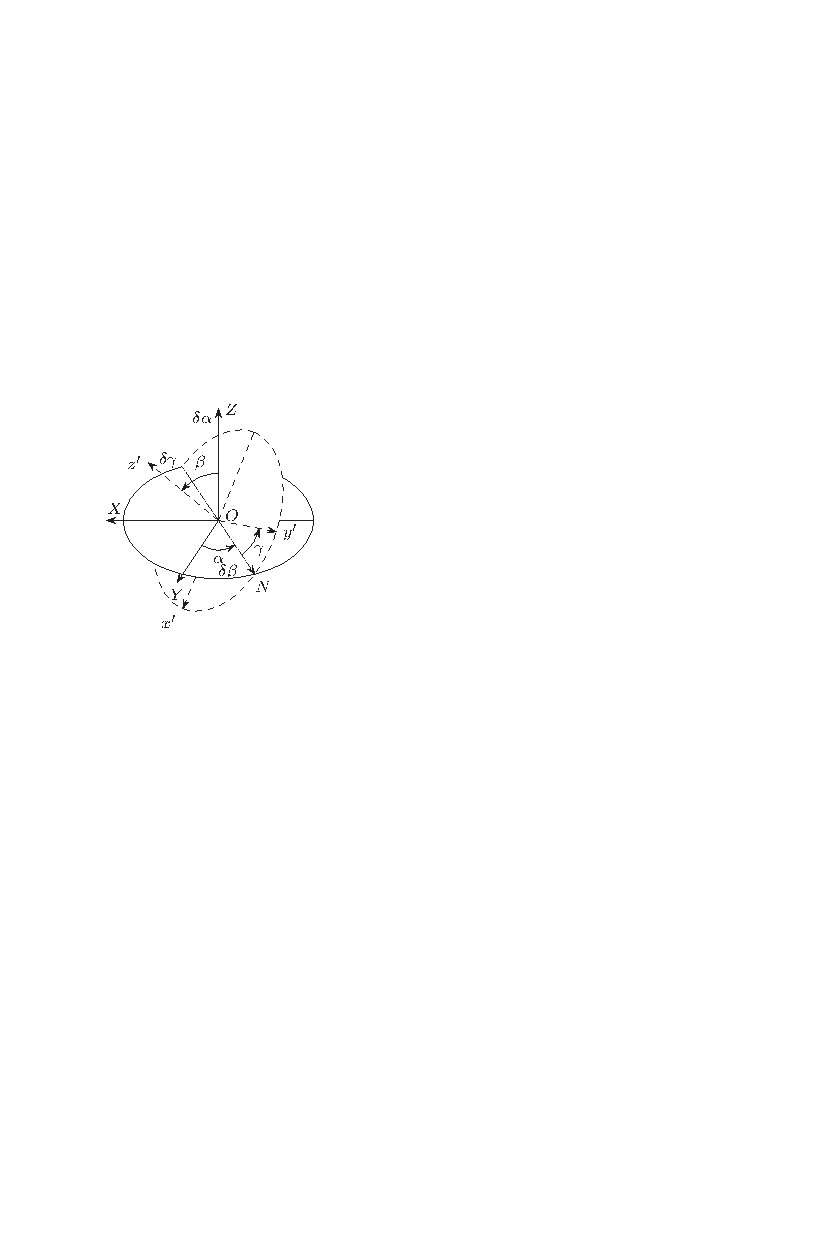
\includegraphics[scale=1.2]{fig}\caption{FIG.20}\label{Fig.20}
\end{wrapfigure}







It is evident that the angles $\alpha$ and $\beta$ are the spherical polar angles $\phi$ and $\theta$ of the new $ z' $-axis with respect to the $ xyz $ axes: $ \alpha = \phi, \beta = \theta $.

In accordance with this manner of rotating the axes, the matrix of the complete transformation is equal to the product of three matrices \eqref{58.3}and \eqref{58.4}:
\[ \hat{U}(\alpha,\beta,\gamma)=\hat{U}_z(\gamma)\hat{U}_y(\beta)\hat{U}_z(\alpha) \]
By direct multiplication of the matrices we finally obtain
\begin{equation}\label{58.6}
\hat{U}(\alpha,\beta,\gamma)=\left( \begin{array}{cc}
\cos(\beta/2)\e^{\i(\alpha+\gamma)/2}&\sin(\beta/2)\e^{-\i(\alpha-\gamma)/2}\\
-\sin(\beta/2)\e^{\i(\alpha-\gamma)/2}&\cos(\beta/2)\e^{-\i(\alpha+\gamma)/2}
\end{array}\right).
\end{equation}



Spinors of higher ranks are, by definition, transformed as products of components of a spinor of rank one. In physical applications, however, we are interested in the wave functions $\psi_{jm}$ rather than the transformation laws of the spinors themselves.

Let the functions $\psi_{jm}$ ($ m = j, j -1, \dots, -j $) describe, in a coordinate system $ xyz $, a state having a definite value of the angular momentum $ j $, and $\psi_{jm}$ the same state for the axes $ x'y'z' $; in the first case $ m $ is the value of $ j_z $, and in the second case $ m' $ is the value of $ j_{z'} $. The two sets of functions are connected by linear relations, which we write in the form
\begin{equation}\label{58.7}
\psi_{jm}=\sum_{m'}D_{m'm}^{(f)}\left(\alpha,\beta,\gamma\right)\psi_{jm'}
\end{equation}
The coefficients $ D_{m'm}^{(j)} $ form a matrix of order $ 2j + 1 $ with respect to $ m' $ and $ m $, called the \textit{finite-rotation matrix} $\hat{D}^{(j)}$; its elements are functions of the angles $ \alpha,\beta,\gamma $ of rotation of the system $ x'y'z' $ relative to $ xyz $.

The finite-rotation matrix can be built up by means of the spinor representation of the functions $\psi_{jm}$. For $ j = 1/2$, the two functions $ \psi_{1/2m}(m = \pm1/2) $ form a covariant spinor of rank $ 1 $. According to \eqref{56.13}, its transformation from $ x'y'z' $ to $ xyz $ is effected by the matrix $\hat{U}$ \eqref{58.6}, so that $ \hat{D}^{(1/2)} = \hat{U} $.\footnote{Note that the matrix indices in \eqref{58.7} are placed in the order that corresponds to multiplying the columns of the matrix $ \hat{D}^{(j)} $ by the functions $\psi_{jm'}$ arranged in a row. In the symbolic notation, \eqref{58.7} would have to be written $ \psi_{jm} = (\psi_j'\hat{D}^{(j)})_m $ in accordance with \eqref{56.13}.
} Its elements may be written
\[ D_{m'm}^{1/2}=\e^{\i m'\gamma}d_{m'm}^{(\beta)\e^{\i m\alpha} \]
where
\begin{equation}\label{58.8}
d_{m'm}^{1/2}(\beta)=\begin{tabular}{c|cc}
\diagbox{$ m' $}{$ m $} & $ 1/2 $&$ -1/2 $\\
\hline
$ 1/2 $ & $ \cos(\beta/2) $ & $ \sin(\beta/2) $,\\
$ -1/2 $ & $ -\sin(\beta/2) $ & $ \cos(\beta/2) $.
\end{tabular}
\end{equation}


For any value of $ j $, the functions $\psi_{jm}$ are related to the components of a symmetrical covariant spinor of rank $ 2j $ by \eqref{57.6}. The transformation matrix for the components of a spinor of rank $ 2j $ is the product of $ 2j $ matrices $ \hat{D}^{(1/2)} $, each acting on one of the spinor indices. Carrying out the multiplication and returning to the functions $\psi_{jm}$, we find their transformation matrix:
\begin{equation}\label{58.9}
D^{(j)}_{m'm}(\alpha,\beta,\gamma)=\e^{\i m'\gamma}d_{m'm}^{(j)}\beta\e^{\i m\alpha},
\end{equation}
the functions $ d_{m'm}^{(j)} (\beta) $ being given by\footnote{The calculations are described by A. R. Edmonds, \textit{Angular Momentum in Quantum Mechanics}, Princeton, 1957. The definition of the functions$ d_{m'm}^{(j)}$ by \eqref{58.9} differs from that used in Edmonds’s book by the interchange of $\alpha$ and $\gamma$, this being the more natural treatment in the approach given here.
}
\begin{multline}\label{58.10}
d_{m'm}^{(j)}(\beta)=\left[\frac{(j+m')!(j-m')!}{(j+m)!(j-m)!} \right]^{1/2}\left(\cos\frac{\beta}{2} \right)^{m'+m}\times\\
\times\left(\sin\frac{\beta}{2} \right)^{m'-m}P_{j-m'}^{(m'-m,m'+m)}(\cos\beta),
\end{multline}
where
\begin{multline}\label{58.11}
P_n^{(a,b)}(\cos\beta)=\frac{(-1)^n}{2^nn!}(1-\cos\beta)^{-\alpha}(1+\cos\beta)^{-b}\times\\
\times\left(\frac{d}{d\cos\beta} \right)^n\left[(1-\cos\beta)^{a+n}(1+\cos\beta)^{b+n} \right]
\end{multline}
are called \textit{Jacobi polynomials}.\footnote{See \S e of the Mathematical Appendices, formula (e.11), for the relation between these polynomials and the hypergeometric series.
} We may note that
\begin{equation}\label{58.12}
P_n^{(a,b)}(-\cos\beta)=(-1)^nP_n^{(b,a)}(\cos\beta).
\end{equation}


The functions $ d_{m'm}^{(j)} $ possess a number of symmetry properties which might be derived from the expressions \eqref{58.11} and \eqref{58.12}, but it is simpler to obtain them directly from the definition as coefficients in the rotational transformation.

The matrix $ \hat{D}^{(j)} $ is unitary, being the matrix of a rotational transformation. Since the transformation inverse to the rotation ($ \alpha,\beta,\gamma $) is the rotation ($ -\gamma,-\beta,-\alpha $), we have for the real matrix $ \hat{d}^{(j)} $ the relations
\begin{equation}\label{58.13}
d_{m'm}^{(j)}(-\beta)=d_{m'm}^{(j)}(\beta)
\end{equation}


The following equations are also valid:
\begin{equation}\label{58.14}
d_{m'm}^{(j)}(\beta)=d_{-m,-m'}^{(j)}(\beta)
\end{equation}
\begin{equation}\label{58.15}
\begin{split}
d_{m'm}^{(j)}(\pi)&=(-1)^{j+m}\delta_{m',-m},\\
d_{m'm}^{(j)}(-\pi)=(-1)^{j-m}&\delta_{m',-m},\quad d_{m'm}^{(j)}(0)=\delta_{m'm}.
\end{split}
\end{equation}
When $ j = 1/2 $ these are evident from \eqref{58.8}; the generalization to arbitrary $ j $ is evident from the manner of construction of the transformation matrix, described above.

A rotation through an angle $ \pi-\beta $ can be carried out as two successive rotations through $\psi$ and $ -\beta $:
\[ d_{m'm}^{(j)}(\pi-\beta)=\sum_{m''}d_{m'm''}^{(j)}(\pi)d_{m''m}^{(j)}(-\beta)=(-1)^{j-m'}d_{-m'm}^{(j)}(-\beta), \]
or, using \eqref{58.13},
\begin{equation}\label{58.16}
d_{m'm}^{(j)}(\pi-\beta)=(-1)^{j-m'}d_{m,-m'}^{(j)}(-\beta).
\end{equation}
The result of two rotations about the same axis is independent of the sequence in which they occur. We must therefore arrive at the same result by carrying out the rotations through $ -\beta $ and $ \pi $ in the opposite order. Comparison of the result with \eqref{58.16} gives the relation
\begin{equation}\label{58.17}
d_{m'm}^{(j)}(\beta)=(-1)^{m'-m}d_{-m',-m}^{(j)}(\beta).
\end{equation}
From \eqref{58.17}, \eqref{58.14} and \eqref{58.13}, it follows that
\begin{equation}\label{58.18}
d_{m'm}^{(j)}(\beta)=(-1)^{m'-m}d_{mm'}^{(j)}(\beta)=(-1)^{m'-m}d_{m'm}^{(j)}(-\beta).
\end{equation}


Using \eqref{58.13}–\eqref{58.18}, we can deduce various symmetry properties of the complete matrix elements $ D_{m'm}^{(j)} $. In particular, the complex conjugate function is given by
\begin{equation}\label{58.19}
D_{m'm}^{(j)*}(\alpha,\beta,\gamma)=D_{m'm}^{(j)}(-\alpha,\beta,-\gamma)=(-1)^{m'-m}D_{-m',-m}^{(j)}(\alpha,\beta,\gamma).
\end{equation}


Mathematically, the matrices $ \hat{D}^{(j)} $ give the unitary irreducible representations of the rotation group having dimension $ 2j + 1 $ (see \S98 below). Hence we have immediately the orthonormality relation
\begin{equation}\label{58.20}
\int D_{m_1'm_1}^{(j_1)*}(\alpha,\beta,\gamma)D_{m_2'm_2}^{(j_2)}(\alpha,\beta,\gamma)\frac{\d\omega}{8\pi^2}=\frac{1}{2j_1+1}\delta_{j_1j_2}\delta_{m_1m_2}\delta_{m_1'm_2'},
\end{equation}
where $ \d\omega = \sin \beta \d\alpha \d\beta \d\gamma $.

The orthogonality of the functions with respect to the suffixes $ m $ and $ m' $ is ensured by the factor $ \exp\{\i(m\alpha+m'\gamma) \} $; that with respect to the index $ j $ arises from the functions $ d_{m'm}^{(j)} $, for which we have
\begin{equation}\label{58.21}
\int_{0}^{\pi}d_{m'm}^{(j_1)}(\beta)d_{m'm}^{(j_2)}(\beta)\frac{\sin\beta\d\beta}{2}=\frac{1}{2j_1+1}\delta_{j_1j_2}.
\end{equation}


Lastly, we shall give for reference the expressions for the functions for various particular values of the parameters. For $ j = 1 $, we have
\begin{equation}\label{58.22}
d_{m'm}^{(1)}(\beta)=\begin{tabular}{c|ccc}
\diagbox{$ m' $}{$ m $} & $ 1 $ & $ 0 $ & $ -1 $\\
\hline
$ 1 $ & $ \frac{1}{2}(1+\cos\beta) $ & $ \frac{1}{\sqrt{2}}\sin\beta $ & $ \frac{1}{2}(1-\cos\beta), $\\
$ 0 $ &$ -\frac{1}{\sqrt{2}}\sin\beta $ & $ \cos\beta $ & $ \frac{1}{\sqrt{2}}\sin\beta, $\\
$ -1 $ & $ \frac{1}{2}(1-\cos\beta) $ & $ -\frac{1}{\sqrt{2}}\sin\beta $ & $ \frac{1}{2}(1+\cos\beta). $
\end{tabular}
\end{equation}

For integral $ j = l $ and $ m' = 0 $, formulae \eqref{58.10} and \eqref{58.11} give
\begin{equation}\label{58.23}
d_{0m}^{(l)}(\beta)=(-1)^md_{m0}^{(l)}(\beta)=(-1)^m\sqrt{\frac{(l-m)!}{(l+m)!}}P_l^m(\cos\beta).
\end{equation}
The derivation of this formula is easily seen from the original definition \eqref{58.7}. We shall assign the values of the functions $\psi_{jm'}$. on the right of \eqref{58.7} to the $ z $-axis, on which (for $ j = l $)
\begin{equation}\label{58.24}
Y_{lm'}(\bm{n}_{z'})=\i^l\sqrt{\frac{2l+1}{4\pi}}\delta_{m'0}.
\end{equation}
 The function $\psi_{jm}$ on the left is then the spherical harmonic function $ Y_{lm}(\beta, \alpha) $ of the spherical polar angles $ \phi\equiv\alpha $, $ \theta\equiv\beta $ giving the direction of the $ z' $-axis. Substitution of \eqref{58.24} in \eqref{58.7} leads to
\begin{equation}\label{58.25}
Y_{lm}(\beta,\alpha)=\i^l\sqrt{\frac{2l+1}{4\pi}}D_{0m}^{(l)}(\alpha,\beta,\gamma),
\end{equation}
which is equivalent to \eqref{58.23}.

Lastly, there is the following expression for the function with the maximum possible value of $ m $ or $ m' $:
\begin{multline}\label{58.26}
d_{jm}^{(j)}(\beta)=(-1)^{j-m}d_{mj}^{(j)}=\\
=\left[\frac{(2j)!}{(j+m)!(j-m)!} \right]^{1/2}\left(\cos\frac{\beta}{2} \right)^{j+m}\left(\sin\frac{\beta}{2} \right)^{j-m}.
\end{multline}

\section{Partial polarization of particles}\label{Partial polarization of particles}
By a suitable choice of the direction of the $ z $-axis, we can always cause one component (e.g. $\psi^2$) of a given spinor $\psi^\lambda$, the wave function of a particle with spin $ 1/2 $, to vanish. This is evident from the fact that a direction in space is determined by two quantities (angles), i.e. the number of disposable parameters is just equal to the number of quantities (the real and imaginary parts of the complex $\psi^2$) which it is desired to make zero.

Physically this means that, if a particle with spin $ 1/2 $ (for definiteness, we shall speak of an electron) is in a state described by a spin wave function, then there is a direction in space in which the component of the particle spin has the definite value $ \sigma=1/2 $. We can say that in such a state the electron is \textit{completely polarized}.

There are also, however, states of an electron which may be said to be \textit{partially polarized}. Such states are not described by wave functions but only by density matrices, i.e. they are mixed states (with respect to spin) (see \S\ref{The density matrix}).

The spin or \textit{polarization} density matrix of an electron is a spinor $ \rho^{\lambda\mu} $ of rank two normalized by the condition
\begin{equation}\label{59.1}
\rho^\lambda{}_\lambda=\rho^1{}_1+\rho^2_2=1
\end{equation}
and satisfying the “Hermitian” condition
\begin{equation}\label{59.2}
(\rho^\lambda{}_\mu)^*=\rho^\mu{}_\lambda.
\end{equation}
For a pure (i.e. completely polarized) spin state of the electron the spinor $ \rho^\lambda{}_\mu $ reduces to a product of components of the wave function $\psi^\lambda$:
\begin{equation}\label{59.3}
\rho^\lambda{}_\mu=\psi^\lambda(\psi^\mu)^*.
\end{equation}


The diagonal components of the density matrix determine the probabilities of the values $ +1/2 $ and $ -1/2 $ of the $ z $-component of the electron spin. The mean value of this component is therefore
\[ \bar{s}_z=\frac{1}{2}(\rho^1{}_1-\rho^2{}_2), \]
or, using \eqref{59.1},
\begin{equation}\label{59.4}
\rho^1{}_1=\frac{1}{2}+\bar{s}_z,\quad\rho^2{}_2=\frac{1}{2}-\bar{s}_z.
\end{equation}


In a pure state the mean value of the quantities $ s_\pm = s_x \pm \i s_y $ is calculated as
\[ \bar{s}_+=\psi^{\lambda*}\hat{s}_+\psi^\lambda,\quad\bar{s}_-=\psi^{\lambda*}\hat{s}_-\psi^\lambda. \]
Since, according to \eqref{55.6} and \eqref{55.7}, the operators $\hat{s}_\pm$ are given by the matrices
\[ \bar{s}_+=\left(\begin{array}{cc}
0&1\\
0&0
\end{array}\right),\quad\bar{s}_-=\left( \begin{array}{cc}
0&0\\
1&0
\end{array}\right), \]
we find that
\[ \bar{s}_+=\psi^{1*}\psi^2,\quad\bar{s}_-\psi^{2*}\psi^1. \]
Accordingly we have in a mixed state
\begin{equation}\label{59.5}
\rho^1{}_2=\bar{s}_-,\quad\rho^2{}_1=\bar{s}_+.
\end{equation}
Using the Pauli matrices, formulae \eqref{59.4} and \eqref{59.5} can be combined as
\begin{equation}\label{59.6}
\rho^\lambda{}_{\mu}=\frac{1}{2}(\delta^\lambda{}_\mu+2\hat{\bm{\sigma}}^\lambda{}_\mu\bar{\bm{s}}).
\end{equation}


Thus all the components of the polarization density matrix of the electron are expressed in terms of the mean values of components of its spin vector. In other words, the real vector $ \bar{\bm{s}} $ entirely determines the polarization properties of a particle with spin $ 1/2 $. In the limit of complete polarization one of the components of this vector (with an appropriate choice of the directions of the axes) is $ 1/2 $ and the other two are zero. In the opposite case of an unpolarized state all three components are zero. In the general case of an arbitrary partial polarization and any choice of the coordinate system we have $ 0\leqslant\rho\leqslant1 $, where
\[ \rho=2(\bar{s}_x^2+\bar{s}_y^2+\bar{s}_z^2)^{1/2} \]
is a quantity which may be called the degree of polarization of the electron.

For a particle of arbitrary spin $ s $, the density matrix is a spinor $ \rho^{\lambda\mu\dots}{}_{\rho\sigma\dots} $ of rank $ 4s $, symmetrical in the first $ 2s $ and the last $ 2s $ indices and satisfying the conditions
\begin{equation}\label{59.7}
\rho^{\lambda\mu\dots}{}_{\lambda\mu\dots}=1,
\end{equation}
\begin{equation}\label{59.8}
\left(\rho^{\lambda\mu\dots}{}_{\rho\sigma\dots} \right)^*=\rho^{\rho\sigma\dots}{}_{\lambda\mu\dots}.
\end{equation}
To calculate the number of independent components of the density matrix, we note that, among the possible sets of values of the indices $ \lambda,\mu,\dots $ (or $ \rho,\sigma,\dots $) there are only $ 2s + 1 $ which are essentially different. Using also the fact that the components of the spinor $ \rho^{\lambda\mu\dots}{}_{\rho\sigma\dots} $ are related by \eqref{59.7}, we find that the number of different components is $ (2s + 1)^2- 1 = 4s (s + 1) $. Although these components are complex, the relation \eqref{59.8} shows that this does not increase the total number of independent quantities describing the state of partial polarization of the particle, which is therefore $ 4s (s+ 1) $.\footnote{When these quantities are given, so are the mean values of the components of the vector $ \bm{s} $ and all their powers and products $ 2, 3, \dots, 2s $ at a time, which do not reduce to lower powers (see \S\ref{The spin operator}, Problem 3).
} For comparison, it may be remarked that the state of complete polarization of the particle is described by only $ 4s $ quantities (the $ 2s + 1 $ complex components of the wave function $\psi^{\lambda\mu\dots}$, related by one normalization condition and containing one common phase which is unimportant in the description of the state).

Like any spinor of rank $ 4s $, the spinor $ \rho^{\lambda\mu\dots}{}_{\rho\sigma\dots} $ is equivalent to a set of irreducible tensors of ranks $ 4s, 4s - 2, \dots, 0 $. In the present case there is only one tensor of each rank, since, on account of the symmetry properties of the spinor $ \rho^{\lambda\mu\dots}{}_{\rho\sigma\dots} $, each contraction of it can be carried out in only one way: with respect to any one of the indices $ \lambda, \mu, \dots, $ and one of $  \rho, \sigma,\dots $. In addition, the scalar (tensor of rank $ 0 $) does not appear, reducing to unity by virtue of the condition \eqref{59.7}.

\section{Time reversal and Kramers’ theorem}\label{Time reversal and Kramers’ theorem}
The symmetry of motion with respect to a change in the sign of the time is expressed in quantum mechanics by the fact that, if $\psi$ is the wave function of a stationary state of the system, the “time-reversed” wave function (which we denote by $\psi^{\mathrm{rev}}$) describes a possible state with the same energy. At the end of \S\ref{The fundamental properties of Schr\"odinger's equation} it has been pointed out that $ \psi^{\mathrm{rev}} $ is the same as the complex conjugate function $ \psi^* $. In this simple form the statement applies to wave functions where the spin of particles is neglected. When spin is present, a refinement is necessary.

Let us take the wave function of a particle of spin $ s $ in the form of the contravariant spinor $ \psi^{\lambda\mu\dots} $ (of rank $ 2s $). On taking the complex conjugate function $ \psi^{\lambda\mu\dots*} $ we obtain a set of quantities which are transformed as components of a covariant spinor. Hence the operation of time reversal corresponds to a change from the wave function $\psi^{\lambda\mu\dots}$ to a new wave function whose covariant components are given by
\begin{equation}\label{60.1}
\psi^{\mathrm{rev}}_{\lambda\mu\dots}=\psi^{\lambda\mu\dots*}.
\end{equation}


For a given set of values of the indices $ \lambda, \mu, \dots, $ the components of covariant and contravariant spinors correspond to values of the angular-momentum component which differ in sign. In terms of the functions $\psi_{s\sim}$ therefore, time reversal corresponds to a change from $\psi_{s\sigma}$ to $ \psi_{s,-\sigma} $, as it should, since a change in the sign of the time changes the direction of the angular momentum. The exact relation is given by \eqref{60.1}:
\begin{equation}\label{60.2}
\psi^{\mathrm{rev}}_{s,-\sigma}=\psi^*_{s\sigma}(-1)^{s-\sigma}.
\end{equation}
Thus the change $ \psi_{s\sigma}\to\psi_{s\sigma}^* $ required by the operation of time reversal signifies the change\footnote{Note that the rule for the complex conjugate of a spherical harmonic function, according to \eqref{28.9}, coincides with the general rule \eqref{60.3}.
}
\begin{equation}\label{60.3}
\psi_{s\sigma}\to\psi_{s,-\sigma}(-1)^{s-\sigma}
\end{equation}


When this operation is repeated, we have
\[\psi_{s\sigma}\to\psi_{s,-\sigma}(-1)^{s-\sigma}\to\psi_{s\sigma}(-1)^{s-\sigma}(-1)^{s+\sigma}=\psi_{s\sigma}(-1)^{2s}. \]



Thus a twofold time reversal restores the wave function to its original value only if the spin is integral; if the spin is half-integral, the sign of the wave function is changed.

Let us consider an arbitrary system of interacting particles. The orbital and spin angular momenta of such a system are not in general separately conserved when relativistic interactions are taken into account. Only the total angular momentum $ \bm{J} $ is conserved. If there is no external field, each energy level of the system has $ (2J + 1) $-fold degeneracy. When an external field is applied, the degeneracy is removed. The question arises whether the degeneracy can be removed completely, i.e. so that the system has only simple levels. This is closely related to the symmetry with respect to time reversal.

In classical electrodynamics the equations are invariant with respect to a change in the sign of the time, if the electric field is left unchanged and the sign of the magnetic field is reversed.\footnote{See, for example, \textit{Fields}, \S17, and the end of \S111 below.} This fundamental property of motion must be preserved in quantum mechanics. Hence, not only in a closed system but in any external electric field (there being no magnetic field), there is symmetry with respect to time reversal.

The wave functions of the system are spinors $ \psi^{\lambda\mu\dots} $, whose rank $ n $ is twice the sum of the spins sa of all the particles ($ n = 2 \sum s_a $); this sum may not be equal to the total spin $ S $ of the system.

According to what was said above, we can assert that, in any electric field, the wave function and its time reversal must correspond to states with the same energy. If a level is non-degenerate, it is necessary that these states should be identical, i.e. the corresponding wave functions must be the same apart from a constant factor (both, of course, being expressed as similar (covariant or contravariant) spinors).

We write $ \psi^{\mathrm{rev}}_{\lambda\mu\dots}=C\psi_{\lambda\mu\dots} $ or, by \eqref{60.1},
\begin{equation}\label{60.4}
\psi^{\lambda\mu\dots*}=C\psi_{\lambda\mu\dots},
\end{equation}
where $ C $ is a constant.

Taking the complex conjugate of both sides of this equation, we obtain
\[ \psi^{\lambda\mu\dots}=C^*\psi^*_{\lambda\mu\dots} .\]
We lower the indices on the left-hand side of the equation and correspondingly raise them on the right. This means that we multiply both sides of the equation by $ g_{\alpha\lambda}g_{\beta\mu\dots} $ and sum over the indices $ \lambda,\mu,\dots $; on the right-hand side we must use the fact that
\[ g_{\alpha\lambda}g_{\beta\mu\dots}=(-1)^ng^{\lambda\alpha}g^{\mu\beta}\dots \]
As a result we have
\[ \psi_{\lambda\mu\dots}=C^*(-1)^n\psi^{\lambda\mu\dots*}. \]
Substituting $ \psi^{\lambda\mu\dots*} $ from \eqref{60.4}, we find
\[ \psi_{\lambda\mu\dots}=(-1)^nCC^*\psi_{\lambda\mu\dots}. \]
This equation must be satisfied identically, i.e. we must have $ (-1)^nCC^* = 1 $. Since, however, $ |C|^2 $ is always positive, it is clear that this is possible only for even $ n $ (i.e. for integral values of the sum $ \sum s_a $). For odd $ n $ (half-integral values of $ \sum s_a $) the condition \eqref{60.4} cannot be fulfilled.\footnote{When the sum $ \sum s_a $ is integral (or halt-integral), all possible values of the total spin $ S $ of the system are also integral (or half-integral).
}

Thus we reach the result that an electric field can completely remove the degeneracy only for a system with an integral value of the sum of the spins of the particles. For a system with a half-integral value of this sum, in an arbitrary electric field, all the levels must be doubly degenerate, and complex conjugate spinors correspond to two different states with the same energy\footnote{If the electric field possesses a high (cubic) symmetry, fourfold degeneracy may occur (see \S99, including the Problem).
} (H. A. Kramers 1930).

One further, mathematical, comment may be made. A relation of the form \eqref{60.4} with a real constant $ C $ is mathematically the condition that the components of the spinor may be put in correspondence with a set of real quantities, and may be called the condition for the spinor to be “real”.\footnote{It is meaningless to call the spinor real in the literal sense, since complex conjugate spinors have different laws of transformation.
} The impossibility of fulfilling the condition \eqref{60.4} for odd $ n $ signifies that no real quantity can correspond to a spinor of odd rank. For even $ n $, on the other hand, the condition \eqref{60.4} can be satisfied, and $ C $ can be real. In particular, a real vector can correspond to a symmetrical spinor of rank two if the condition \eqref{60.4} is satisfied with $ C = 1 $:
\[\psi^{\lambda\mu*}=\psi_{\lambda\mu}  \]
(as is easily seen by means of \eqref{57.8} and \eqref{57.9}). The condition \eqref{60.4} with $ C = 1 $ is in fact the condition for a symmetrical spinor of any even rank to be “real”.
